\appendix

\chapter{Algorithm Pseudo Codes}
\label{ap:pseudo-codes}


\begin{algorithm}[htbp]
\DontPrintSemicolon
\caption{Standard \gls{acr:ppo} using \gls{acr:gae}, shown for a representative agent $i$}
\label{alg:ppo}
\BlankLine
Initialize policy parameters $\theta^i$ and value parameters $\phi^i$\;
\For{$k = 1, 2, \dots, N_{\mathrm{iter}}$}{
  Run $\pi_{\theta^i_{\mathrm{old}}}$ in the environment to collect a set of trajectories $\mathcal{D}_k$\;
  Compute $\widehat{AV}^i_t$ for all $t$ via \gls{acr:gae} from the current value function $V^i_{\phi^i}$\;
  Update $\theta^i$ by maximizing $J^{\mathrm{CLIP},i}(\theta^i)$ for $N_{\mathrm{ep}}$ epochs with minibatch size $B$\;
  Update $\phi^i$ by minimizing the value mean-squared error for $N_{\mathrm{ep}}$ epochs with minibatch size $B$\;
  Update the policy $\theta^i_{\mathrm{old}} \leftarrow \theta^i$\;
}
\textbf{end for}
\end{algorithm}


    
\begin{algorithm}[htbp]
\DontPrintSemicolon
\caption{\gls{acr:ippo} with parameter sharing \citep{dewitt2020independent}}
\label{alg:ippo}
\BlankLine
Initialize shared policy parameters $\theta$ and shared value parameters $\phi$\;
\For{$k = 1, 2, \dots, N_{\mathrm{iter}}$}{
  Run the shared policy $\pi_{\theta_{\mathrm{old}}}$ in the environment for every agent $i$ to collect the joint trajectories $\mathcal{D}_k$\;
  Compute $\widehat{AV}^i_t$ for all agents $i$ and all $t$ via \gls{acr:gae} from the local critic $V_{\phi}(o^i_t)$\;
  Update $\theta$ by maximizing $J^{\mathrm{CLIP}}(\theta)$ over the pooled experience of all agents for $N_{\mathrm{ep}}$ epochs with minibatch size $B$\;
  Update $\phi$ by minimizing the value mean-squared error of $V_{\phi}(o^i_t)$ for $N_{\mathrm{ep}}$ epochs with minibatch size $B$\;
  Update the policy $\theta_{\mathrm{old}} \leftarrow \theta$\;
}
\textbf{end for}
\end{algorithm}



\begin{algorithm}[H]
\DontPrintSemicolon
\caption{\gls{acr:mappo} with parameter sharing \citep{yu2022surprising}}
\label{alg:mappo}
\BlankLine
Initialize shared policy parameters $\theta$ and shared value parameters $\phi$\;
\For{$k = 1, 2, \dots, N_{\mathrm{iter}}$}{
  Run the shared policy $\pi_{\theta_{\mathrm{old}}}$ in the environment for every agent $i$ to collect the joint trajectories $\mathcal{D}_k$\;
  Compute $\widehat{AV}^i_t$ for all agents $i$ and all $t$ via \gls{acr:gae} from the centralized critic $V_{\phi}(\mathbf{o}_t)$\;
  Update $\theta$ by maximizing $J^{\mathrm{CLIP}}(\theta)$ over the pooled experience of all agents for $N_{\mathrm{ep}}$ epochs with minibatch size $B$\;
  Update $\phi$ by minimizing the value mean-squared error of $V_{\phi}(\mathbf{o}_t)$ for $N_{\mathrm{ep}}$ epochs with minibatch size $B$\;
  Update the policy $\theta_{\mathrm{old}} \leftarrow \theta$\;
}
\textbf{end for}
\end{algorithm}





\newpage
\chapter{Reference Baseline Descriptions}
\label{ap:baselines}

This appendix documents every reference baseline implemented and evaluated in this work, including several that support the analysis without entering the main results. Two of the baselines act as the main performance anchors of the study. Specifically, BS-Optimized is the heuristic reference that defines the performance gap and \gls{acr:cppo} is the centralized \gls{acr:rl} ceiling. The remaining baselines fix the reference scale from Random at its
lower anchor up to BS-Optimized at the upper bound. 

\paragraph{\textbf{Random.}} The random policy ignores the state entirely and draws each
warehouse's per-\gls{acr:sku} action independently from a uniform distribution on
$[-1,1]$ at every period. It performs no calibration and therefore has no tunable
parameter. Since the demand-centered mapping of \autoref{subsec:action-design} turns
a zero action into an order equal to the observed demand, a uniform action scatters
orders around that demand level without regard to inventory or pipeline. The
resulting return marks the zero point of the normalized score against which every
skilled policy is measured.

\paragraph{\textbf{ConstantOrder.}} The constant-order policy places the same order quantity in
every period irrespective of the current state. To obtain a reasonable constant quantity that applies to all \glspl{acr:sku} and warehouses equally, it first
estimates the mean home-region demand $\hat\mu^D_{ik}$ of each warehouse and \gls{acr:sku} over $50$ pilot episodes and then orders the rounded quantity $q_{ik}=\operatorname{round}(\alpha\,\hat\mu^D_{ik})$ at every step, where the single
multiplier $\alpha$ is shared across all warehouses and \glspl{acr:sku}. The
multiplier is tuned by a grid sweep over $\{0.05,0.10,\dots,2.0\}$, and the value
with the highest mean return on training-mode rollouts is locked for the held-out
evaluation.

\paragraph{\textbf{Base-Stock Policies.}} The remaining four non-learned baselines are base-stock policies that share one
order-up-to rule and differ only in how the target level $S_{ik}$ is set for
warehouse $i$ and \gls{acr:sku} $k$. Each such
policy tracks the inventory position $I_{ikt}+I^{\mathrm{tr}}_{ikt}$ and orders the quantity that raises this position back to the
target level $S_{ik}$ such that the order in each timestep is given by 
\begin{equation}
\label{eq:bs-order}
  q_{ikt}=\max\!\big\{0,\ S_{ik}-I_{ikt}-I^{\mathrm{tr}}_{ikt}\big\}.
\end{equation}
Each level $S_{ik}$ is kept separate for every warehouse and \gls{acr:sku} because the cost-optimal level
depends jointly on the local demand scale and the \gls{acr:sku} weight such that a shared
level would understate the heuristic ceiling and inflate the apparent advantage of
the learned policies.

\paragraph{\textbf{BS-Newsvendor.}} The newsvendor policy fixes each target level
analytically from the true demand parameters and therefore acts as an oracle that an
online controller cannot reproduce. For warehouse $i$ and \gls{acr:sku} $k$ it reads
the home-region mean demand $\mu^D_{ik}$ of \autoref{eq:expected-demand}, forms the
expected lead-time demand $L_{ik}\mu^D_{ik}$, and adds a safety term proportional to
the Poisson lead-time standard deviation,
\begin{equation}
\label{eq:bs-newsvendor}
  S_{ik}=L_{ik}\,\mu^D_{ik}+z\,\sqrt{L_{ik}\,\mu^D_{ik}}.
\end{equation}
This level matches the steady-state initialization of \autoref{eq:initial-inventory}
and leaves the safety factor $z$ as its only free parameter. The factor is tuned by a
grid sweep over $\{0,0.25,\dots,6.0\}$ and the value with the highest mean
training-mode return is retained for evaluation.

\paragraph{\textbf{BS-Adaptive.}} The adaptive policy is adopted from \citet{Neale2009} and replaces the oracle parameters with
statistics estimated online and therefore shows how a base-stock rule performs once
the true rates are unknown. At each period, it maintains the empirical mean
$\bar D^{H}_{ikt}$ and variance $V^{H}_{ikt}$ of the home-region demand observed over
the most recent $H$ periods and forms the time-varying target
\begin{equation}
\label{eq:bs-adaptive}
  S_{ikt}=L_{ik}\,\bar D^{H}_{ikt}+z\,\sqrt{L_{ik}\,V^{H}_{ikt}}.
\end{equation}
In contrast to the newsvendor policy, it estimates the demand variance from data
rather than assuming the Poisson identity and orders nothing before the first demand is observed. Both the safety factor $z$ and the window width $H$ are tuned jointly
over the grid $z\in\{0,0.25,\dots,6.0\}$ and $H\in\{5,10,20,30,40,50,100\}$ and the
pair with the highest mean training-mode return is retained for evaluation.

\paragraph{\textbf{BS-Optimized.}} The optimized policy discards every analytical formula and
searches directly for the target levels that minimize simulated cost. It treats the
full set of $W\times K$ levels as continuous variables on $[0,U]$ with $U=200$ and
fits them jointly by Gaussian-process \gls{acr:bo} \citep{Frazier2018}, which approximates the target level as 
\begin{equation}
\label{eq:bs-optimized}
  S^{\star}\approx\arg\min_{S\in[0,U]^{W\times K}}
  \frac{1}{M}\sum_{m=1}^{M}\mathrm{TSCC}_m(S),
\end{equation}
where $\mathrm{TSCC}_m(S)$ is the realized total cost of rollout $m$ under the base-stock
policy with levels $S$ and $M=50$. The search uses $50$ random initial points
followed by $300$ guided evaluations after which $S^{\star}$ is fixed and evaluated
on the held-out seed. Because this policy knows the dynamics, faces no learning
constraint, and is optimized on the same distribution it is evaluated on, it provides the upper anchor of the normalized score.

\paragraph{\textbf{BS-Independent.}} The independent policy runs the same simulation
optimization as BS-Optimized but removes all joint search and therefore isolates the value of
optimizing the warehouses together. It optimizes one warehouse at a time by iterated
best response such that in round $r$ warehouse $i$ updates
its own levels while the other warehouses stay fixed at $S^{(r)}_{-i}$. The optimization objective is thus given by
\begin{equation}
\label{eq:bs-independent}
  S^{(r+1)}_{i}=\arg\min_{S_i\in[0,U]^{K}}
  \frac{1}{M}\sum_{m=1}^{M}\sum_{t}C_{it}\big(S_i,S^{(r)}_{-i}\big).
\end{equation}
Each warehouse is therefore scored on its own per-period cost $C_{it}$ rather than the network cost, which reproduces the incentive faced by an independent agent under the agent-scoped reward of. The update uses $100$ \gls{acr:bo} evaluations per warehouse,
repeats for three rounds, and is initialized from the newsvendor levels of
\autoref{eq:bs-newsvendor} at $z=1$. The gap between this policy and BS-Optimized
measures how much the jointly optimized reference gains from coordinating the levels
rather than setting them as mutual best responses.

\paragraph{CPPO.} \Gls{acr:cppo} is the only learned baseline and serves as the
\gls{acr:rl} ceiling. A single \gls{acr:ppo} agent reads the concatenated joint
observation $\mathbf{o}_t$ of all warehouses and emits the joint action
$\mathbf{a}_t\in\mathcal{A}$ such that the network is driven by one controller rather than
$W$ cooperating agents. This collapses the cooperative game into a single-agent
problem and removes partial observability, environment non-stationarity, and
multi-agent credit assignment at once. It is trained and tuned with the same
optimization and hyperparameter-search protocol as the \gls{acr:marl} algorithms and
therefore carries no baseline-specific tuning of its own.



\newpage
\chapter{Real-World Freight Data}
\label{ap:real-data}

\begin{figure}[h]
\centering
\includegraphics[width=1.0\linewidth, height=0.6\textheight, keepaspectratio]{images/warehouse_costs.png}
\caption[Variable freight cost against distance in the real-world data]{%
Per-weight variable freight cost against shipping distance for the inbound route (top) and the outbound route (bottom) in the real-world freight dataset. Red markers show the points used to calibrate the environment (inbound $\approx 1.0$ per unit weight and outbound $\approx 0.5$ per unit weight at $\approx 500$ km and $\approx 0.05$ per unit weight for the $50$ km home leg).}
\label{fig:freight-data}
\end{figure}







\newpage
\chapter{Heterogeneity gap for \gls{acr:ippo-ps} and \gls{acr:mappo-ps}}
\label{ap:heterogeneity-gap}

\begin{table}[ht]
\centering
\small
\renewcommand{\arraystretch}{1.2}
\caption[Heterogeneous performance gap (IPPO-PS)]{Gap of
\gls{acr:ippo-ps} on each heterogeneous variant, reported as the percentage by
which episode cost exceeds the BS-Optimized reference.}
\label{tab:het-gap-ippo}
\begin{tabular}{@{}l c c c c@{}}
\toprule
 & \multicolumn{2}{c}{\gls{acr:ippo-ps} Gap (\%)} & \gls{acr:cppo} (\%) & \\
\cmidrule(lr){2-3}
\textbf{Variant} & Transfer & Re-tuned & Re-tuned & Gap above \gls{acr:cppo} (\%) \\
\midrule
SKU      & 43.0 & 10.7 & $-6.1$ & $16.7^{***}$\\
Demand   & 17.0 &  9.1 & $-0.0$ & $\phantom{0}9.2^{***}$\\
Cost     &  7.9 &  7.7 & $\phantom{-}1.2$ & $\phantom{0}6.5^{***}$\\
Combined & 48.4 & $-2.3$ & $-2.2$ & $-0.1^{\text{\,n.s.}}$\\
\bottomrule
\end{tabular}

\smallskip
{\footnotesize $*** $ $p < 0.001$; $** $ $p < 0.01$; $* $ $p < 0.05$; n.s. denotes not significant.}
\end{table}


\begin{table}[ht]
\centering
\small
\renewcommand{\arraystretch}{1.2}
\caption[Heterogeneous performance gap (MAPPO-PS)]{Gap of \gls{acr:mappo-ps} on each heterogeneous variant, reported as the
percentage by which episode cost exceed the BS-Optimized reference.}
\label{tab:het-gap}
\begin{tabular}{@{}l c c c c@{}}
\toprule
 & \multicolumn{2}{c}{\gls{acr:mappo-ps} Gap (\%)} & \gls{acr:cppo} (\%) & \\
\cmidrule(lr){2-3}
\textbf{Variant} & Transfer & Re-tuned & Re-tuned & Gap above \gls{acr:cppo} (\%) \\
\midrule
SKU      & 30.9 & 10.7 & $-6.1$ & $16.8^{***}$\\
Demand   & 15.7 &  8.7 & $-0.0$ & $\phantom{0}8.7^{***}$\\
Cost     &  7.4 &  7.9 & $\phantom{-}1.2$ & $\phantom{0}6.7^{***}$\\
Combined & 38.2 & $-2.1$ & $-2.2$ & $\phantom{0}0.1^{\text{\,n.s.}}$\\
\bottomrule
\end{tabular}

\smallskip
{\footnotesize $*** $ $p < 0.001$; $** $ $p < 0.01$; $* $ $p < 0.05$; n.s. denotes not significant.}
\end{table}






















\chapter{Reward Decomposition}
\label{ap:reward-decomposition}

This appendix derives the CREDIT intervention of \autoref{sec:interventions}.
It shows that splitting the per-warehouse reward into one channel per \gls{acr:sku} lowers
the variance of the policy gradient and sharpens per-\gls{acr:sku} credit while leaving the
optimum of the pooled baseline unchanged.

\paragraph{\textbf{Setup.}} A single parameter-shared policy controls one warehouse through a
factored action $a_t=(a_t^1,\dots,a_t^S)$ with one coordinate per \gls{acr:sku}. The policy is
a diagonal Gaussian, so it factorizes across the $S$ coordinates,
\begin{equation}
\pi_\theta(a_t\mid s_t)=\prod_{s=1}^{S}\pi_\theta^{s}(a_t^{s}\mid s_t),
\qquad
\ln\pi_\theta(a_t\mid s_t)=\sum_{s=1}^{S}\ln\pi_\theta^{s}(a_t^{s}\mid s_t).
\label{eq:factor}
\end{equation}
Each factor $\pi_\theta^{s}$ is the marginal that sets \gls{acr:sku} $s$'s order, and the joint
log-probability is the sum of the per-coordinate log-probabilities. The action side of the update
therefore already separates by \gls{acr:sku}. The rest of this appendix shows that the reward side
separates the same way and that pairing the two yields a lower-variance estimator with the same
fixed points.

\paragraph{\textbf{Additive cost decomposition.}} The per-warehouse reward is the sum of the
\glspl{acr:sku}' negative costs, $r_t=\sum_{s} r_t^{s}$, where $r_t^{s}$ gathers \gls{acr:sku}
$s$'s holding, lost-sales, outbound, and inbound cost. The equality is exact because the
non-separable fixed per-order shipment cost is zero in every environment.
Linearity of the discounted sum and of the expectation then propagates the same split to the
return, the value, and the advantage,
\begin{gather}
G_t^{s}=\sum_{k\ge 0}\gamma^{k} r_{t+k}^{s},\qquad
G_t=\sum_{s} G_t^{s},\\[2pt]
V^{s}(s_t)=\mathbb{E}_\pi\!\big[G_t^{s}\mid s_t\big],\qquad
V(s_t)=\sum_{s} V^{s}(s_t),\\[2pt]
\widehat{AV}_t^{s}=G_t^{s}-V^{s}(s_t),\qquad
\widehat{AV}_t=\sum_{s} \widehat{AV}_t^{s}.
\label{eq:advdecomp}
\end{gather}
Each per-\gls{acr:sku} advantage $\widehat{AV}_t^{s}$ is thus measured against its own baseline $V^{s}$ such that the critic must carry $S$ value heads rather than one.

\paragraph{\textbf{Pooled policy gradient (baseline).}} The policy-gradient theorem \citep{Sutton1999} together with
\eqref{eq:factor} and \eqref{eq:advdecomp} gives
\begin{align}
\nabla_\theta J
&=\mathbb{E}\!\left[\sum_t \nabla_\theta\ln\pi_\theta(a_t\mid s_t)\,\widehat{AV}_t\right]\\
&=\mathbb{E}\!\left[\sum_t\sum_{s}
\nabla_\theta\ln\pi_\theta^{s}(a_t^{s}\mid s_t)
\Big(\underbrace{\widehat{AV}_t^{s}}_{\text{own}}
+\underbrace{\textstyle\sum_{s'\ne s}\widehat{AV}_t^{s'}}_{\text{cross terms}}\Big)\right].
\label{eq:pooled}
\end{align}
Thus, each coordinate's score is multiplied by the \emph{total} advantage such that it also absorbs the other \glspl{acr:sku}' advantages. The next two steps show that these cross terms contribute zero in expectation.

\paragraph{\textbf{Zero-mean cross terms.}} For a diagonal policy, $a_t^{s}$ is conditionally
independent of $a_t^{-s}=(a_t^{s'})_{s'\ne s}$ given $s_t$. Additionally, the per-coordinate score is zero-mean,
\begin{equation}
\mathbb{E}_{a_t^{s}\sim\pi_\theta^{s}}\!\big[\nabla_\theta\ln\pi_\theta^{s}(a_t^{s}\mid s_t)\big]
=\nabla_\theta\!\int \pi_\theta^{s}(a^{s}\mid s_t)\,da^{s}=\nabla_\theta 1=0 .
\label{eq:scorezero}
\end{equation}
It follows that for any $f(s_t,a_t^{-s})$ that does not depend on $a_t^{s}$, it must hold, 
\begin{equation}
\mathbb{E}\!\big[\nabla_\theta\ln\pi_\theta^{s}(a_t^{s}\mid s_t)\,f(s_t,a_t^{-s})\big]=0 .
\label{eq:cfbaseline}
\end{equation}
Setting $f=\sum_{s'\ne s}\widehat{AV}_t^{s'}$ then removes the cross terms from \eqref{eq:pooled} and pairs
each coordinate with its own advantage,
\begin{equation}
\boxed{\;\nabla_\theta J
=\mathbb{E}\!\left[\sum_t\sum_{s}
\nabla_\theta\ln\pi_\theta^{s}(a_t^{s}\mid s_t)\,\widehat{AV}_t^{s}\right]\;}
\label{eq:decomp}
\end{equation}
The bias dropped in this step is exactly
$\sum_{s'\ne s}\mathbb{E}\big[\nabla_\theta\ln\pi_\theta^{s}\,\widehat{AV}_t^{s'}\big]$, which is
nonzero only when \gls{acr:sku} $s$'s action changes another \gls{acr:sku}'s reward. Within a step
there is no such change as the shared per-order shipment cost is zero and warehouse capacity
is unbounded. Therefore, \eqref{eq:cfbaseline} cancels the immediate cross terms exactly. Across steps,
$a_t^{s}$ reaches the other \glspl{acr:sku} only through the shared next state, which essentially is a second-order effect whose residual vanishes at any stationary point where the advantages average to zero. The optimum thus never moves.

\paragraph{\textbf{Score under the parameterization used.}} The argument above needs only that the
score of the Gaussian is zero-mean, which the actual parameterization satisfies. The log standard deviations
$\ell_s$ form a single state-independent vector that is shared across states and warehouses, whereas the
means $\mu_s(s_t)$ are the network output and $\sigma_s=e^{\ell_s}$. A diagonal Gaussian factorizes for any $\sigma$, which is why \eqref{eq:factor} and every step above are unchanged. The scores are given by,
\begin{equation}
\partial_{\theta_\mu}\ln\pi^s=\frac{a^s-\mu_s}{\sigma_s^{2}}\,\partial_{\theta_\mu}\mu_s,
\qquad
\partial_{\ell_s}\ln\pi^s=\frac{(a^s-\mu_s)^2}{\sigma_s^{2}}-1,
\end{equation}
and depend only on \gls{acr:sku} $s$'s own residual and are zero-mean under $\pi^s$, which is everything that \eqref{eq:cfbaseline} requires.

\paragraph{\textbf{Variance.}} Both estimators are unbiased for the same within-step gradient such that they differ only in variance. Writing the per-\gls{acr:sku} score as
$g_s=\nabla_\theta\ln\pi_\theta^{s}$ and treating the injected cross-\gls{acr:sku} noise as
uncorrelated with coordinate $s$'s own term,
\begin{equation}
\mathrm{Var}\!\big(g_s \widehat{AV}_t\big)
=\mathrm{Var}\!\Big(g_s\textstyle\sum_{s'}\widehat{AV}_t^{s'}\Big)
\;\ge\;
\mathrm{Var}\!\big(g_s \widehat{AV}_t^{s}\big),
\end{equation}
because the pooled form adds every other \gls{acr:sku}'s zero-mean advantage to coordinate $s$
without changing its mean. The excess is dominated by the heaviest \gls{acr:sku}, whose cost noise
would otherwise reach all $S$ coordinates at once. Decomposition confines that noise to the
coordinate that produced it.

\paragraph{\textbf{PPO surrogate.}} The factored gradient has a matching \gls{acr:ppo} objective.
Because the policy is diagonal, the probability ratio factorizes as $\rho_t=\prod_s \rho_t^{s}$ with
$\rho_t^{s}=\pi_\theta^{s}/\pi_{\theta_{\mathrm{old}}}^{s}$, and the per-coordinate credit of
\eqref{eq:decomp} carries over by clipping each coordinate's own ratio against its own advantage as,
\begin{equation}
L(\theta)=\hat{\mathbb{E}}\!\left[\sum_{s}
\min\!\Big(\rho_t^{s}\,\widehat{AV}_t^{s},\;
\operatorname{clip}(\rho_t^{s},1-\epsilon,1+\epsilon)\,\widehat{AV}_t^{s}\Big)\right].
\label{eq:ppo-factored}
\end{equation}
This is the factored form of the clipped objective $J^{\mathrm{CLIP},i}$ of \eqref{eq:ppo}, and at
$S=1$ it collapses to that single-head surrogate exactly.

\paragraph{\textbf{Critic loss.}} The advantages the actor consumes come from a critic with one head
per \gls{acr:sku}. Each head regresses on its own bootstrapped return
$\hat G_t^{s}=\widehat{AV}_t^{s}+V^{s}(s_t)$, and is trained by the summed squared error,
\begin{equation}
L^{V}(\phi)=\hat{\mathbb{E}}\!\left[\sum_{s=1}^{S}\big(V_\phi^{s}(s_t)-\hat G_t^{s}\big)^{2}\right],
\label{eq:vloss}
\end{equation}
which is the factored analogue of the pooled value loss $\hat{\mathbb{E}}\big[(V_\phi(s_t)-\hat G_t)^2\big]$. It reduces to that loss at $S=1$ and reproduces it in aggregate through $\sum_s V^{s}=V$ and $\sum_s \hat G_t^{s}=\hat G_t$. Summing
rather than averaging the heads trains each at the rate of an independent scalar critic and keeps
the actor-critic balance of \eqref{eq:ppo-factored}. Averaging would instead rescale the value term
by $1/S$.

\paragraph{\textbf{Stationary points unchanged.}} The decomposition above leaves the solution set intact.
If the heads are consistent, $\sum_s V^{s}=V$, then $\widehat{AV}_t^{s}=0$ for all $s$ implies
$\widehat{AV}_t=0$ such that the pooled and factored gradients vanish together. At such a fixed point the
dropped cross-\gls{acr:sku} bias is zero as well since it is built from the same advantages.
Decomposition thus changes only the variance and the credit attribution of the gradient and not
its stationary points. Thus, the optimal policy and the unweighted evaluation objective coincide with those of the pooled baseline.




















\newpage
\chapter{Per-SKU Self-Attention Architecture}
\label{ap:sku-attention}

This appendix details the actor and critic backbone of the actor and critic backbone of ATTENTION, which builds one block per \gls{acr:sku} directly into the network so that the policy treats the \glspl{acr:sku}
symmetrically before any cross-\gls{acr:sku} interaction.

\paragraph{\textbf{Forward pass.}} The architecture interprets the flat
observation as one or more repeated warehouse blocks. It uses one block for a
local actor, $1+W$ blocks for the global \gls{acr:mappo} critic, and $W$ blocks
for the \gls{acr:cppo} joint observation. Within each warehouse block the per-\gls{acr:sku} columns are gathered into one token per \gls{acr:sku}, $x_1,\dots,x_K$, where the gather handles both contiguous and strided feature groups such as the pipeline. A single shared linear layer projects every token to the embedding width as,
\begin{equation}
\label{eq:attn-proj}
  z_k = W_{\mathrm{in}}\,x_k + b_{\mathrm{in}} \in \mathbb{R}^{d_{\mathrm{model}}},
  \qquad k = 1,\dots,K .
\end{equation}
A transformer encoder then applies multi-head self-attention across the
\gls{acr:sku} tokens of that block such that each token is updated by a learned
weighted combination of all tokens as,
\begin{equation}
\label{eq:attn-mhsa}
  [\tilde z_1,\dots,\tilde z_K] = \mathrm{Encoder}\big([z_1,\dots,z_K]\big).
\end{equation}
The attention runs within each warehouse block with weights shared across blocks,
so a \gls{acr:mappo} critic attends inside each warehouse rather than across
warehouses. The attended tokens are flattened and concatenated with the
non-per-\gls{acr:sku} context features $c$ (i.e., the warehouse-identity one-hot and the aggregate features). A small \gls{acr:mlp} head $g$ then maps the result to the output as follows,
\begin{equation}
\label{eq:attn-head}
  y = g\big([\,\tilde z_1,\dots,\tilde z_K,\ c\,]\big),
\end{equation}
which is the vector of per-\gls{acr:sku} action means in the actor and a single
scalar value in the critic.

\paragraph{\textbf{Fixed configuration.}} The architecture is held fixed rather
than tuned, so that the intervention budget stays symmetric across all
interventions and the matched-capacity control of the next paragraph targets a
single architecture per environment. Specifically, the embedding width is $d_{\mathrm{model}}=64$,
the head count is $n_{\mathrm{heads}}=2$, the encoder feed-forward width is
$\mathrm{ff}_{\mathrm{hidden}}=64$, and the read-out head has hidden sizes $[128]$
for the actor and $[64]$ for the critic. Because the shared projection of
\autoref{eq:attn-proj} and the attention of \autoref{eq:attn-mhsa} are applied
tokenwise with shared weights, the parameter count of the attention stage is
independent of the number of \glspl{acr:sku} and grows only with
$d_{\mathrm{model}}^2$. \autoref{fig:sku-attention-arch} summarizes the forward
pass.



\begin{figure}[H]
\centering
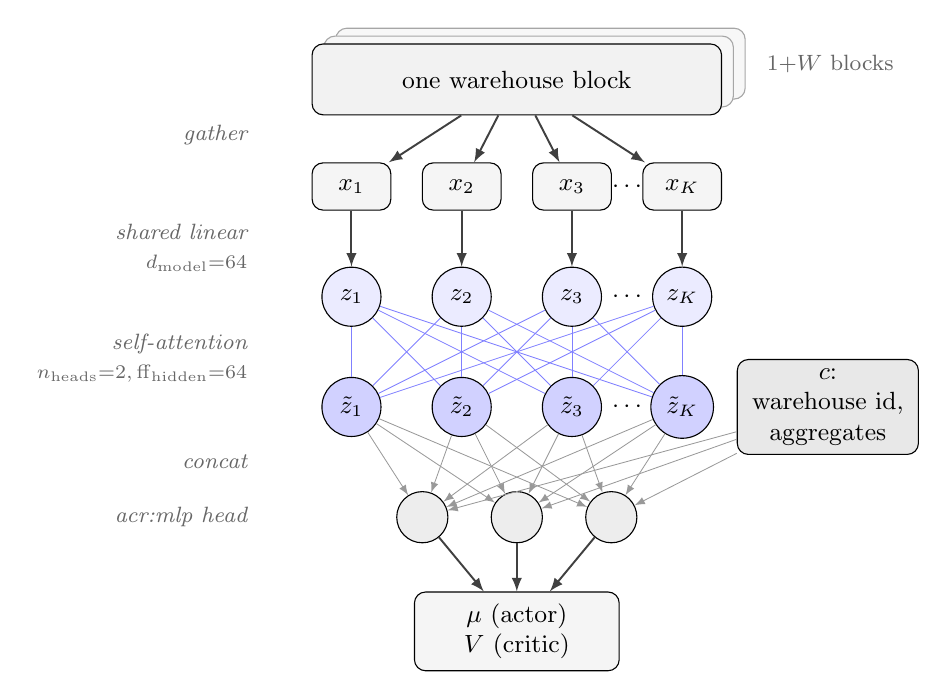
\begin{tikzpicture}[
  >=latex, font=\small,
  block/.style={draw, rounded corners, minimum width=52mm, minimum height=9mm,
                align=center, fill=black!5},
  tok/.style={draw, rounded corners, minimum width=10mm, minimum height=6mm, fill=black!4},
  proj/.style={draw, circle, minimum size=7.5mm, fill=blue!8},
  att/.style={draw, circle, minimum size=7.5mm, fill=blue!18},
  hid/.style={draw, circle, minimum size=6.5mm, fill=black!7},
  ctx/.style={draw, rounded corners, minimum width=23mm, minimum height=11mm,
              align=center, fill=black!9},
  outp/.style={draw, rounded corners, minimum width=26mm, minimum height=10mm,
              align=center, fill=black!4},
  stage/.style={font=\footnotesize\itshape, text=black!60, anchor=east, align=right},
  flow/.style={->, draw=black!75, line width=0.7pt},
  attn/.style={draw=blue!50, line width=0.3pt},
  dense/.style={->, draw=black!40, line width=0.3pt},
]
% repeated warehouse blocks (stacked cards), input at the top
\node[block, fill=black!3, draw=black!35] at (0.30,5.96) {};
\node[block, fill=black!3, draw=black!35] at (0.15,5.86) {};
\node[block] (blk) at (0,5.76) {one warehouse block};
\node[font=\footnotesize, text=black!60, anchor=west] at (3.05,5.96) {$1{+}W$ blocks};
% gathered per-SKU input tokens
\node[tok] (x1) at (-2.1,4.4) {$x_1$};
\node[tok] (x2) at (-0.7,4.4) {$x_2$};
\node[tok] (x3) at ( 0.7,4.4) {$x_3$};
\node[tok] (xK) at ( 2.1,4.4) {$x_K$};
\node at (1.4,4.4) {$\cdots$};
% projected tokens
\node[proj] (z1) at (-2.1,3.0) {$z_1$};
\node[proj] (z2) at (-0.7,3.0) {$z_2$};
\node[proj] (z3) at ( 0.7,3.0) {$z_3$};
\node[proj] (zK) at ( 2.1,3.0) {$z_K$};
\node at (1.4,3.0) {$\cdots$};
% attended tokens
\node[att] (a1) at (-2.1,1.6) {$\tilde z_1$};
\node[att] (a2) at (-0.7,1.6) {$\tilde z_2$};
\node[att] (a3) at ( 0.7,1.6) {$\tilde z_3$};
\node[att] (aK) at ( 2.1,1.6) {$\tilde z_K$};
\node at (1.4,1.6) {$\cdots$};
% context (concatenated alongside the attended tokens)
\node[ctx] (c) at (3.95,1.6) {$c$:\\ warehouse id,\\ aggregates};
% MLP head hidden layer
\node[hid] (h1) at (-1.2,0.2) {};
\node[hid] (h2) at ( 0.0,0.2) {};
\node[hid] (h3) at ( 1.2,0.2) {};
% output
\node[outp] (y) at (0,-1.25) {$\boldsymbol{\mu}$ (actor)\\ $V$ (critic)};
% stage labels with fixed hyperparameters (left)
\node[stage] at (-3.3,5.05) {gather};
\node[stage] at (-3.3,3.62) {shared linear\\[1pt]{\scriptsize$d_{\mathrm{model}}{=}64$}};
\node[stage] at (-3.3,2.22) {self-attention\\[1pt]{\scriptsize$n_{\mathrm{heads}}{=}2, \mathrm{ff}_{\mathrm{hidden}}{=}64$}};
\node[stage] at (-3.3,0.90) {concat};
\node[stage] at (-3.3,0.20) {\gls{acr:mlp} head};
% gather: block -> tokens
\foreach \t in {x1,x2,x3,xK}{ \draw[flow] (blk) -- (\t); }
% shared linear: tokens -> projected
\foreach \i/\z in {x1/z1, x2/z2, x3/z3, xK/zK}{ \draw[flow] (\i) -- (\z); }
% self-attention: all-to-all across SKU tokens
\foreach \s in {z1,z2,z3,zK}{
  \foreach \t in {a1,a2,a3,aK}{ \draw[attn] (\s) -- (\t); }
}
% flatten + concat context -> MLP head
\foreach \s in {a1,a2,a3,aK,c}{
  \foreach \h in {h1,h2,h3}{ \draw[dense] (\s) -- (\h); }
}
% head -> output
\foreach \h in {h1,h2,h3}{ \draw[flow] (\h) -- (y); }
\end{tikzpicture}
\caption[Per-SKU self-attention backbone]{The attention backbone for one
warehouse block, drawn top-down. Per-\gls{acr:sku} tokens are projected, mixed by
multi-head self-attention, concatenated with the context $c$, and read out by an
\gls{acr:mlp} head to the action means $\boldsymbol{\mu}$ (actor) or value $V$
(critic).}
\label{fig:sku-attention-arch}
\end{figure}


